\documentclass[a4paper,12pt]{article}

\usepackage[spanish]{babel}
\usepackage[utf8]{inputenc}
\usepackage[T1]{fontenc}
\usepackage[utf8]{inputenc}
\usepackage{makeidx}
\usepackage{graphicx}
\usepackage{lmodern}
\usepackage{kpfonts}
\usepackage[left=2cm,right=2cm,top=2cm,bottom=2cm]{geometry}
\usepackage{amsmath,amsfonts,amssymb}
\usepackage{hyperref}
\hypersetup{
    colorlinks=true,
    linkcolor=cyan,
    filecolor=magenta,      
    urlcolor=blue,
    pdftitle={titulo},
    pdfpagemode=FullScreen,
    }
\urlstyle{same}

\title{Asignación 2}

\begin{document}

\begin{center}
\par 
\includegraphics[scale=1]{USB} \par
Universidad Simon Bolivar \\ Curso: CI3311 / Sistemas de Base de Datos I \\ Trimestre: Enero-Marzo, 2024 \\ Profesor: Pedro Pérez \\ Estudiante: Junior Miguel Lara Torres - Carnet: 17-10303 \\
\end{center}

\begin{center}
Asignación 2
\end{center}

\begin{itemize}
\item \textbf{Requerimientos de datos}
	
	Link directo, Google Drive - PDF, de los requerimientos. \href{https://drive.google.com/file/d/1WlY4fa3ZEyj-rs8Jd862_azSV6XtuzHy/view?usp=drive_link}{Enlace}.
	
\item \textbf{Diagrama ER-E}

	Link directo al diagrama en LucidChart \href{https://lucid.app/lucidchart/df3ad355-f421-4600-bc67-f57184f6d9bb/edit?viewport_loc=2110%2C-117%2C2560%2C1224%2C0_0&invitationId=inv_
	e8d58044-5d17-4379-acd1-2fb790ad52e4}{Enlace}. O en su defecto a Google Drive - PDF \href{https://drive.google.com/file/d/1u0yD14KliKU6Sydkkrh3dgvys6tM2FqL/view?usp=drive_link}{Enlace}.
\end{itemize}

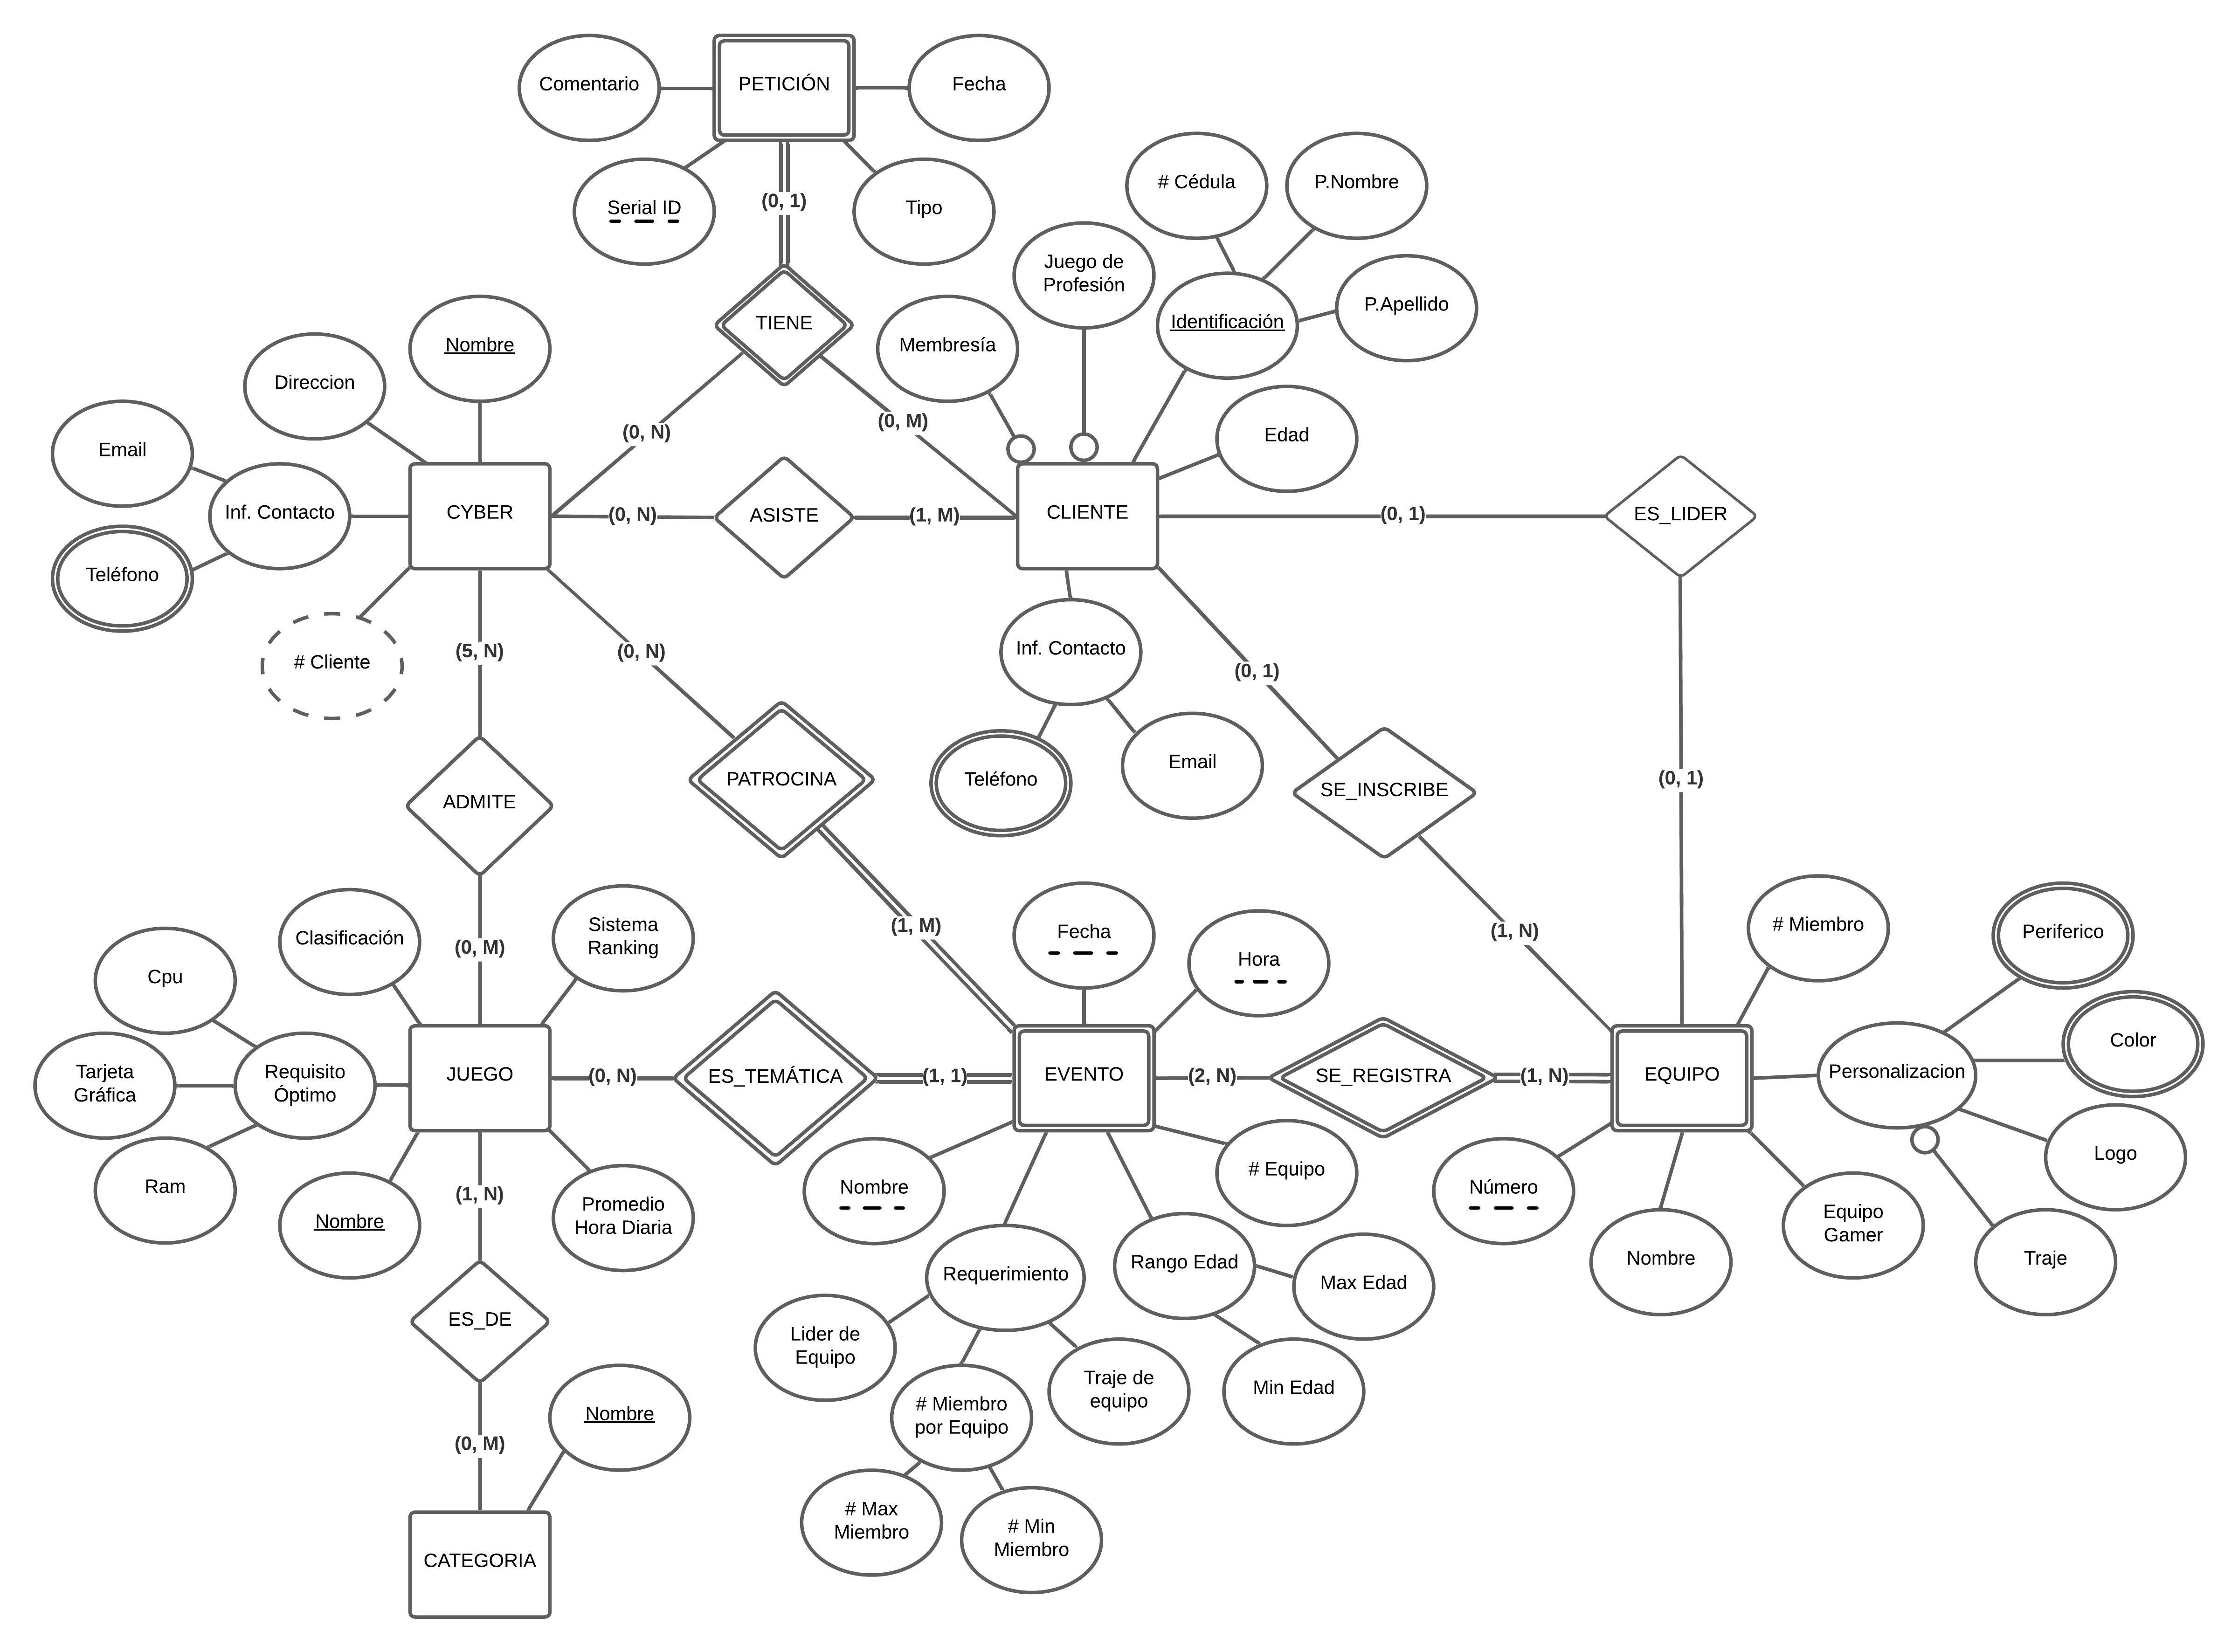
\includegraphics[scale=0.45]{Diagrama Illussions Gamers - Junior Lara.jpeg} $\\~$

\begin{itemize}
\item \textbf{Restricciones Explícitas}

La notación $R(e_1, e_2, ..., e_n)$ describe como cada una de las instancias de entidad $e_1, e_2, ..., e_n$ se relacionan entre sí mediante la relación $R$. Esta notación simplifica el siguiente predicado:$\\ $

$((\forall / \exists) x_1, x_2, ..., x_n | E_1(x_1) \land ... \land E_n(x_n) \land (\exists r_1 | R_1(r_1) : r_1[E_i] = x_i \land ... \land r_1[E_j] = x_j)) \\ $
$: (\exists r_2 | R_2(r) : r_2[E_n] = x_n \land ... \land r_2[E_m] = x_m)\\ $ 
Con $i \neq j \land n \neq m$ y sin una secuencia especifica.$\\ $

A la siguiente expresión$\\ $

$((\forall / \exists) x_1, x_2, ..., x_n | E_1(x_1) \land ... \land E_n(x_n) \land R_1(x_i, ..., x_j) : R_2(x_n, ..., x_m)) \\ $
Con $i \neq j \land n \neq m$ y sin una secuencia especifica. $\\ $

La forma correcta de lectura depende de la interpretación que tengan los verbos usados para las relaciones y los nombres de los tipos de entidades que participen en ella, pero por lo regular es de izquierda a derecha. $\\ $
Por ejemplo, mas adelante verá algo similar a
\begin{itemize}
\item $TIENE(c,p,cy)$ referencia a $"$Un cliente c tiene una petición p en un cyber cy".
\item $SE\_INSCRIBE(c, eq)$ referencia a $"$Un cliente c se inscribe en un equipo eq".
\item $SE\_REGISTRA(eq, ev)$ referencia a $"$Un equipo eq se registra en un evento ev".
\item $ES\_TEMATICA(j, ev)$ referencia a $"$Un juego j es temática de un evento ev".
\item $PATROCINA(cy, ev)$ referencia a $"$Un cyber cy patrocina a un evento ev".
\item $ES\_LIDER(c, eq)$ referencia a $"$Un cliente c es líder de un equipo eq".
\end{itemize}

\begin{enumerate}
\item Para que un evento tenga temática de juego, este juego debe tener un Sistema de Ranking.

$(\forall e, t| EVENTO(e) \land ES\_TEMÁTICA(t):(\exists j| JUEGO(j) \land j.Sistema\_Ranking = TRUE : t[EVENTO] = e \land t[JUEGO] = j))$

\item Todo cliente inscrito en un equipo cumple el mínimo y máximo de edad permitido por el evento.

$(\forall c, eq, ev,| CLIENTE(c) \land EQUIPO(eq) \land EVENTO(ev)\land  SE\_INSCRIBE(c, eq)\land SE\_REGISTRA(eq, ev): ev.Rango\_Edad.Min\_Edad \leq c.Edad \leq ev.Rango\_Edad.Max\_Edad)$ 

\item Todo los miembros de un equipo participante en un evento cumple con la clasificación del juego.

$(\forall c, eq, ev, j| CLIENTE(c) \land EQUIPO(eq) \land EVENTO(ev) \land JUEGO(j)\land SE\_INSCRIBE(c, eq) \land SE\_REGISTRA(eq, ev) \land ES\_TEMATICA(j, ev):c.Edad \geq j.Clasificación )$

\item La fecha de un evento no puede ser un día festivo ni un día lunes.

$(\forall ev | EVENTO(ev):dia\_de\_fecha(ev.fecha) \neq '\text{Lunes}' \land es\_dia\_festivo(ev.Fecha) = FALSE)$
\begin{itemize}
\item Donde $dia\_de\_fecha$ es una función que recibe string en formato 'd/m/a' representando la fecha y retorna un string perteneciente al conjunto \{"Lunes", "Martes", "Miercoles", "Jueves", "Viernes", "Sábado", "Domingo"\}.
\item Donde $es\_dia\_festivo$ es una función que recibe string en formato 'd/m/a' y retorna un boleando indicando si ese string que representa una fecha es un día festivo o no.
\end{itemize}

\item La hora de un evento debe estar entre las 10 y 17 horas.

$(\forall ev | EVENTO(ev):'10:00:00' \leq ev.Hora \leq '17:00:00')$
   
\item Todo equipo admite líder en los equipos si el evento lo admite.

$(\forall eq, ev | EQUIPO(eq) \land EVENTO(ev) \land SE\_REGISTRA(eq, ev)\land$

$ev.Requerimiento.Lider\_de\_Equipo = TRUE: (\exists1! c | CLIENTE(c): ES\_LIDER(c, eq)))$ 
   
\item Todo equipo admite traje en los equipos si el evento lo admite.

$(\forall eq, ev | EQUIPO(eq) \land EVENTO(ev) \land SE\_REGISTRA(eq, ev)\land$

$ev.Requerimiento.Traje\_de\_Equipo = TRUE: eq.Personalizacion.Traje \neq NULL)$ 
   
\item Todo Cyber patrocina eventos con temáticas de juegos que solo estén en su catálogo.

$(\forall cy, ev, j | CYBER(cy) \land EVENTO(ev) \land JUEGO(j) \land PATROCINA(cy, ev)\land$

$ES\_TEMATICA(j, ev): ADMITE(cy, j))$
   
\item Todo Cyber admite peticiones de clientes que solo asisten al mismo.

$(\forall cy,c,p|CYBER(cy)\land CLIENTE(c)\land PETICION(p)\land TIENE(c,p,cy): ASISTE(c, cy))$
   
\item El líder de un equipo debe estar inscrito en el equipo.

$(\forall c, eq | CLIENTE(c) \land EQUIPO(eq) \land ES\_LIDER(c, eq): (\exists!1 si | SE\_INSCRIBE(si) : si[CLIENTE] = c \land si[EQUIPO] = eq))$

\item Los clientes inscritos en el equipo que participa en un evento, deben ser los mismos clientes del Cyber que patrocina el mismo evento.

$(\forall c, eq, ev, cy | CLIENTE(c) \land EQUIPO(eq) \land EVENTO(ev) \land CYBER(cy)\land$

$PATROCINA(cy, ev) \land SE\_REGISTRA(eq, ev) \land SE\_INSCRIBE(c, eq): ASISTE(c, cy))$
    
\item El número total de miembros por equipo respetan los requerimientos descritos por el evento.

$(\forall eq, ev | EQUIPO(eq) \land EVENTO(ev):$

$ev.Requerimiento.\#\_Miembro\_por\_equipo.\#\_Min\_Miembro$

$\leq eq.\#\_Miembro \leq$

$ev.Requerimiento.\#\_Miembro\_por\_equipo.\#\_Max\_Miembro)$
    
\item La cantidad de clientes inscritos en un equipo respecta el mínimo y máximo de miembros por equipo descritos en el evento al cual participa el mismo.

$(\forall eq,ev | EQUIPO(eq) \land EVENTO(ev) \land SE\_REGISTRA(eq, ev):$

$ev.Requerimiento.\#\_Miembro\_por\_equipo.\#\_Min\_Miembro$

$\leq (\sum c |CLIENTE(c) \land SE\_INSCRIBE(c, eq) : 1)\leq$

$ev.Requerimiento.\#\_Miembro\_por\_equipo.\#\_Max\_Miembro)$
\end{enumerate}

$\\ \\ \\ \\ \\ \\ $
\item \textbf{Dominios}
\begin{enumerate}
\item En Cyber
\begin{itemize}
\item Nombre: Cadena de caracteres. 
\item Dirección: Cadena de caracteres.
\item Email: Cadena de caracteres.
\item Teléfono: Cadena de caracteres, con formato "+xx-xxx-xxx-xx-xx" con x un numero decimal.
\item $\#$ Cliente: Numero entero no negativo.
\end{itemize}

\item En Petición
\begin{itemize}
\item Serial ID: Cadena de caracteres de tamaño 9, con formato "xxxx-xxxx" donde x toma valores alfanuméricos.
\item Tipo: Cadena de caracteres perteneciente al conjunto \{"Queja", "Solicitud"\}.
\item Fecha: Cadena de caracteres, con formato "d/m/a" donde d toma valores enteros entre 1 y 31, m toma valores enteros entre 1 y 12, y a toma valores enteros entre 2024 en adelante.
\item Comentario: Cadena de caracteres.
\end{itemize}

\item En Cliente
\begin{itemize}
\item P.Nombre: Cadena de caracteres.
\item P.Apellido: Cadena de caracteres.
\item $\#$ Cédula: Número entero no negativo.
\item Edad: Número entero mayor a 17.
\item Juego de Profesión: Cadena de caracteres que haga referencia a algún juego existente en la vida real.
\item Membresía: Cadera de caracteres, con el formato "Premium x" donde x es un numero entero entre el 0 y el 5.
\item Email: Cadena de caracteres.
\item Teléfono: Cadena de caracteres, con formato "+xx-xxx-xxx-xx-xx" con x un numero decimal.
\end{itemize}

\item En Equipo
\begin{itemize}
\item Número: Numero entero no negativo.
\item Nombre: Cadena de caracteres.
\item Equipo Gamer: Cadena de caracteres que haga referencia a un equipo gamer existente en la vida real.
\item Periférico: Cadena de caracteres que hace referencia un periférico para un equipo gamer en la vida real.
\item Color: Cadena de caracteres perteneciente al conjunto de los colores \{"Azul", "Rojo", "Purpura", ...\}.
\item Logo: Cadena de caracteres que hace referencia a una descripción detallada de un logo en la vida real.
\item Traje: Cadena de caracteres que hace referencia a una descripción detallada de un traje en la vida real.
\item $\#$ Min Miembro: Numero entero no negativo.
\item $\#$ Max Miembro: Numero entero no negativo.
\end{itemize}		
		
$\\ $
\item En Evento
\begin{itemize}
\item Nombre: Cadena de caracteres.
\item Fecha: Cadena de caracteres, con formato "d/m/a" donde d toma valores enteros entre 1 y 31, m toma valores enteros entre 1 y 12, y a toma valores enteros entre 2024 en adelante.
\item Hora: Cadena de caracteres, con formato "xx:xx:xx" donde x es un numero decimal y hace referencia a hora militar.
\item Líder de Equipo: Booleano.
\item $\#$ Min Miembro por equipo: Numero entero no negativo.
\item $\#$ Max Miembro por equipo: Numero entero no negativo.
\item Traje de Equipo: Booleano.
\item $\#$ Min Edad: Numero entero no negativo.
\item $\#$ Max Edad: Numero entero no negativo.
\item $\#$ Equipo: Numero entero no negativo.
\end{itemize}		
		
\item En Juego
\begin{itemize}
\item Nombre: Cadena de caracteres.
\item Clasificación: Numero entero no negativo que pertenece al conjunto de clasificaciones actuales de \href{https://es.wikipedia.org/wiki/Entertainment_Software_Rating_Board "Entertainment Software Rating Board"}{Entertainment Software Rating Board} que se puede describir por \{0(Todas las edades o 6 años o más), 10(10 años o más), 13(13 años o más), 17 (Menores deben tener permiso de un adulto), 18 (Los niños o adolescentes no se les permite comprar, alquilar o jugar/verlas )\}.
\item Sistema de Ranking: Booleano.
\item Promedio hora diaria: Numero entero no negativo.
\item CPU: Cadena de caracteres que hace referencia a una unidad central de procesamiento en la vida real.
\item Tarjeta gráfica: Cadena de caracteres que hace referencia a una Unidad de procesamiento gráfico en la vida real.
\item RAM: Cadena de caracteres que hace referencia a una memoria de acceso aleatorio en la vida real.
\end{itemize}
		
\item En Categoría
\begin{itemize}
\item Nombre: Cadena de caracteres.
\end{itemize}

\end{enumerate}

\end{itemize}
\end{document}